\subsection{Ορισμός ποιότητας εσωτερικού αέρα}


Σύμφωνα με την υπηρεσία προστασίας του περιβάλλοντος της Αμερικής 
(US \linebreak Environmental Protection Agency,EPA),η ποιότητα εσωτερικού αέρα (Indoor Air Quality, IAQ) ορίζεται έως η ποιότητα του αέρα 
μέσα και γύρω από κτίρια και γενικά κατασκευές, ιδιαίτερα σε σχέση με την υγεία και την άνεση των ανθρώπων \cite{USEPA}.

Η ποιότητα του εσωτερικού αέρα σχετίζεται άμεσα σαν έννοια με την ρύπανση του εσωτερικού αέρα (Indoor Air Pollution).
Όμως, η ποιότητα του εσωτερικού χώρου εμπεριέχει και σαν πρωτογενή κομμάτι μελέτη της την σχετική υγρασία και θερμοκρασία του κτιρίου, που είναι περιβαλλοντικές συνθήκες, όπως και την εσωτερική ποιότητα CO2.
Αποτελούν παράγοντες που μπορούν να επηρεάσουν την υγεία και την άνεση των ανθρώπων \cite{10.1371/journal.pone.0305956}, όπως και να επηρεάσουν τους ρύπου που υπάρχουν στον εσωτερικό χώρο 
και να μας δώσουν πληροφορίες για την γενικότερη ποιότητα του συγκεκριμένου εσωτερικού χώρου.
Πρέπει να συμπληρώσουμε εδώ είναι φυσικοί παράγοντες και όχι ρύποι, βρισκόμενοι έτσι πιο κοντά στην έννοια της ποιότητας του εσωτερικού περιβάλλοντος (Indoor Environmental Quality,IEQ) \cite{Piasecki2017264}. 

%Γενική όροι Όπως επίσης και τις έννοιες του συνδρόμου του νοσούντος κτιρίου (Sick Building Syndrome,SBS) ασθένειες σχετικές με κάποιο κτίριο (Building Related Illness,BRI) και πολλαπλή χημική ευαισθησία  (multiple chemical sensitivity MCS)\cite{Ahmed(2019)}


Η ατμοσφαιρική ρύπανση είναι η μόλυνση του εσωτερικού ή του εξωτερικού περιβάλλοντος από οποιονδήποτε χημικό, 
φυσικό ή βιολογικό παράγοντα που αλλοιώνει τα φυσικά χαρακτηριστικά της ατμόσφαιρας \cite{WHODEFINITION}. 
Αποτελεί τον περιβαλλοντικό παράγοντα με την μεγαλύτερη επιβάρυνση στην ανθρώπινη υγεία \cite{WHO2021} και ένας από τους σημαντικότερους παράγοντες επιβάρυνσης της υγείας συνολικά σε παγκόσμιο επίπεδο, 
όπου επιφέρει ανά χρόνο εκατομμύρια ανθρώπινους θανάτους και χρόνων χαμένης υγιούς ζωής, ή όπως ορίζεται, έτη ζωής προσαρμοσμένα στην αναπηρία (Disability-Adjusted Life-Years,DALYs) \cite{Forouzanfar2015}.

 

\subsection{Οι επιπτώσεις της χαμηλής ποιότητας εσωτερικού αέρα παγκόσμια}

Σύμφωνα με αναφορά του Παγκόσμιου οργανισμός υγείας (Π.Ο.Υ.) για το 2016 \cite{WHO2018v2} \cite{WHO2018v3}, υπολογίζεται ότι οι θάνατοι που έχουν σαν αίτιο την ρύπανση του αέρα ανέρχονται παγκόσμια 
στα 8 εκατομμύρια ανθρώπους τον χρόνο. Για την ατμοσφαιρική ρύπανση, 
οι νεκροί ανήλθαν στα 4.2 εκατομμύρια, με το 90\% να είναι σε χαμηλού και μέτριου οικονομικά επιπέδου χώρες (Low and Middle Income countries,LMI countries), 
με την Ελλάδα να μην υπάγεται σε κάποια από αυτές τις χώρες.
Οι ασθένειες που περιλαμβάνει η αναφορά είναι η οξεία λοίμωξη του κατώτερου αναπνευστικού (ALRI), 
ο καρκίνος των πνευμόνων, η χρόνια αποφρακτική πνευμονοπάθεια, η ισχαιμική καρδιοπάθεια και το εγκεφαλικό. 
Οι μη μεταδοτικές ασθένειες ευθύνονται για το 82\% αυτών των θανάτων.

Για τους υπόλοιπους 3.8 εκατομμύρια θανάτους που υπάγονται στην ρύπανση του εσωτερικού αέρα, 
σχεδόν όλοι προέρχονται από χαμηλού και μέτριου οικονομικά επιπέδου χώρες, με μόλις εννιά χιλιάδες να είναι θάνατοι από υψηλού επιπέδου οικονομικά χώρες.
Οι ασθένειες που περιλαμβάνει η αναφορά είναι η οξεία λοίμωξη του κατώτερου αναπνευστικού, ο καρκίνος των πνευμόνων, η χρόνια αποφρακτική πνευμονοπάθεια, 
η ισχαιμική καρδιοπάθεια και το εγκεφαλικό. Οι μη μεταδοτικές ασθένειες ευθύνονται για το 73\% αυτών των θανάτων.
Μία πιο αναλυτική και γενική περίληψη των επιπτώσεων  στην υγεία της κακής ποιότητας αέρας στον εσωτερικό χώρο δίνονται στην \autoref{fig:ISGLOBAL}.


Ο λόγος που προκύπτει τέτοια αναντιστοιχία μεταξύ των πλούσιων και των υπόλοιπων χωρών είναι το γεγονός ότι μεγάλο κομμάτι του πληθυσμού του πλανήτη χρησιμοποιεί 
για το μαγείρεμα ανοιχτές φωτιές ή μη αποτελεσματικές κουζίνες.
Για να λειτουργήσουν, χρειάζεται να χρησιμοποιηθούν στερεά καύσιμα \cite{WHO2025}.
Στην βιβλιογραφία, αυτού του είδους ρύπανση αναφέρεται και έως οικιακή εσωτερική ρύπανση (Household Indoor Pollution, HIP). 
Δυστυχώς, τα νούμερα που περιγράφονται πιο πάνω συνεχίζουν να ισχύουν έως σήμερα \cite{GlobalAir2025}. 

\begin{figure}[b]
    \centering
    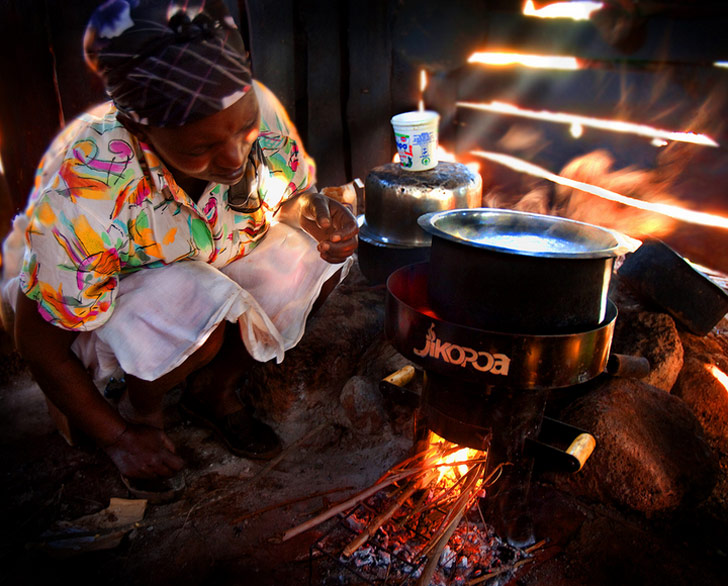
\includegraphics[width=0.8\textwidth]{εικόνες/woman cooking.jpg}
    \caption{Παράδειγμα μαγειρέματος με ανοιχτή φωτιά σε εσωτερικό χώρο \cite{BUSINESSINSIDERAFRICA2022}}
    \label{fig:WomanCooking}
\end{figure}


\begin{figure}[h!]
    \centering
    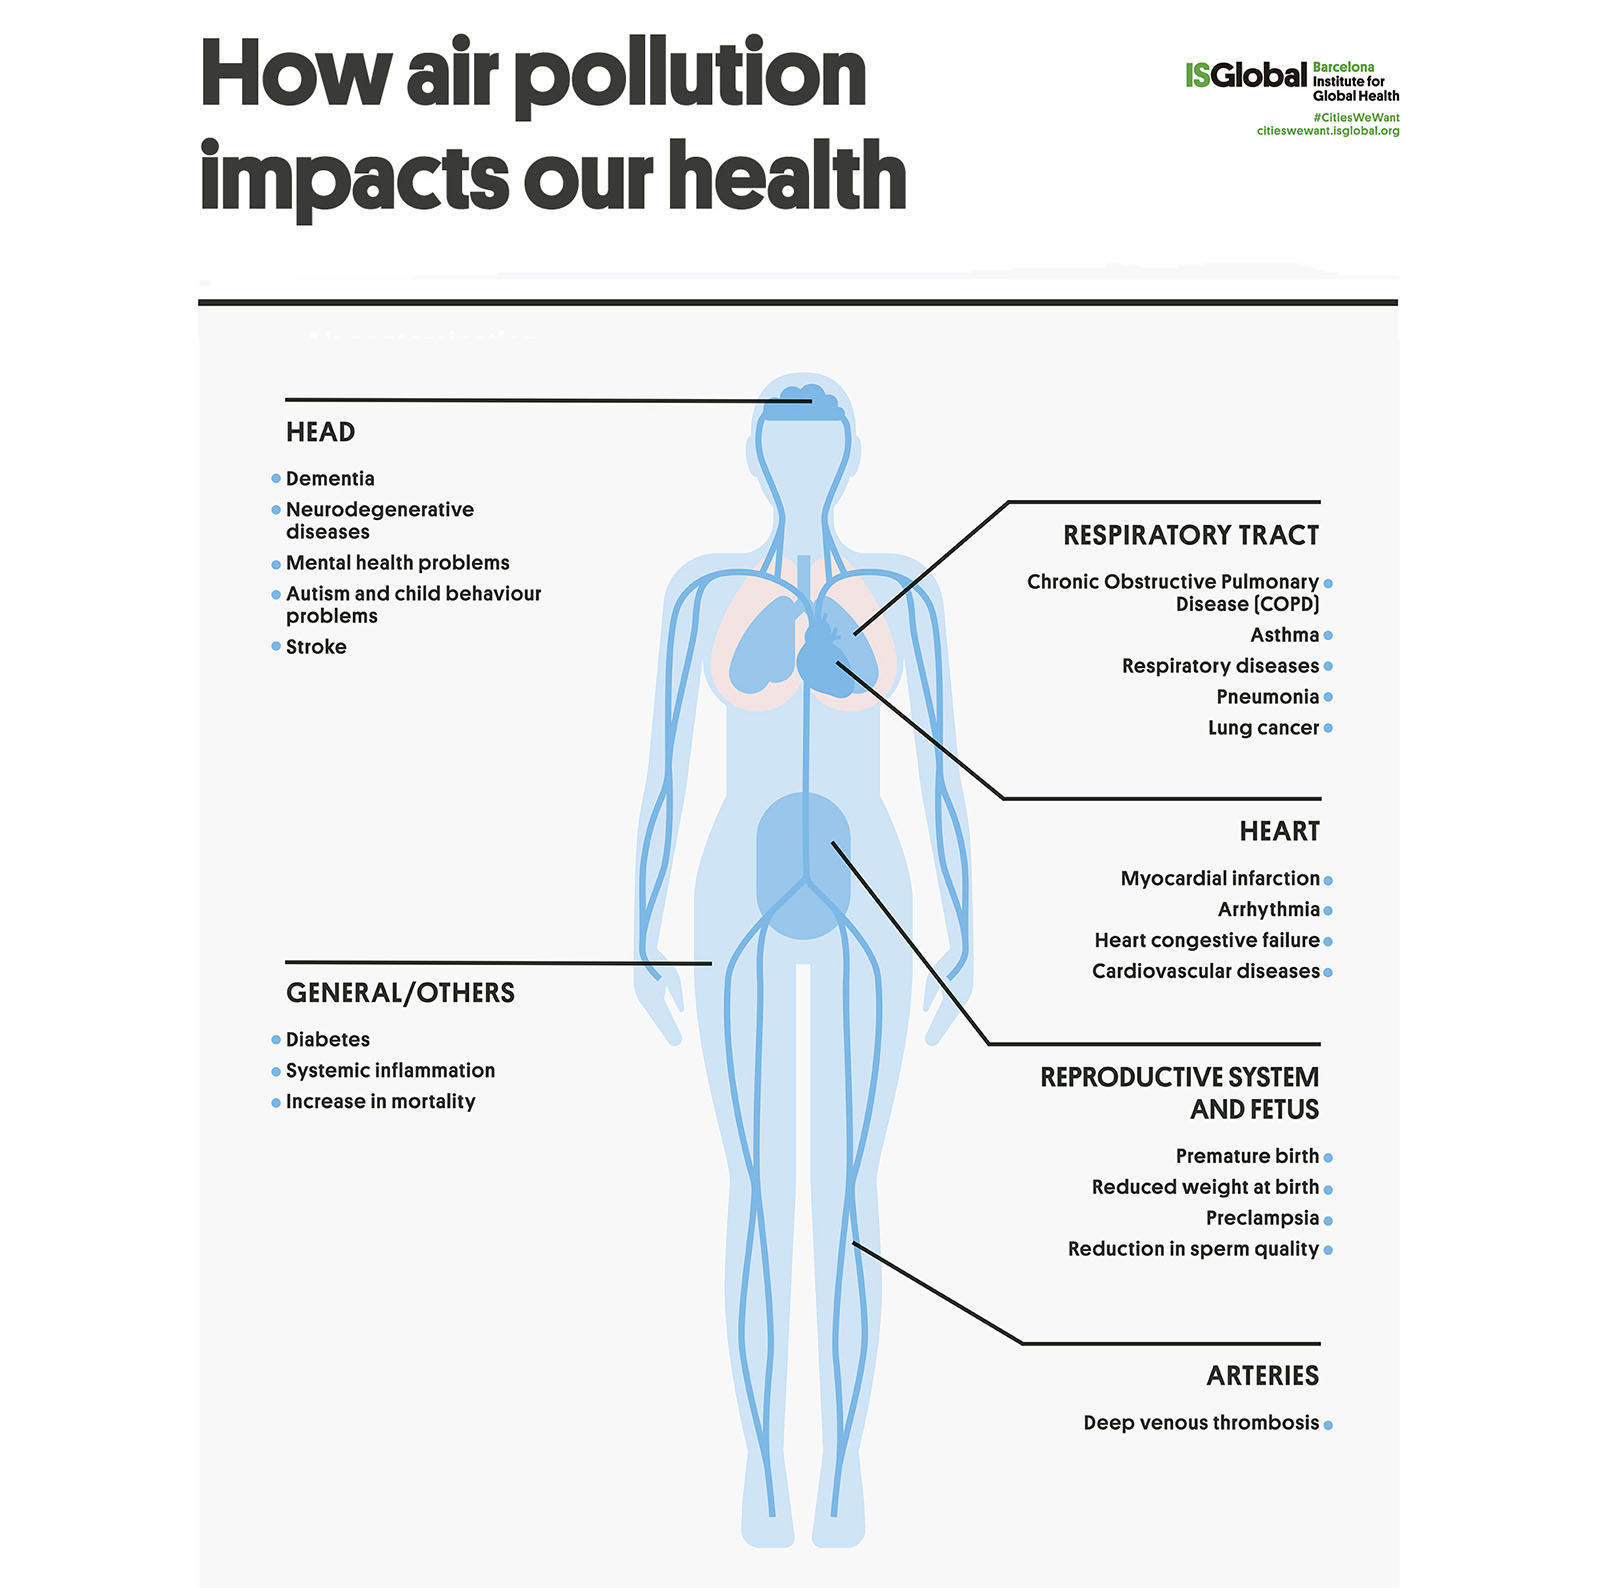
\includegraphics[width=0.8\textwidth]{εικόνες/air pollution body eng copia.jpg}
    \caption{Οι επιπτώσεις των ρύπων στην υγεία \cite{ISGLOBAL2018} }
    \label{fig:ISGLOBAL}
\end{figure}

\FloatBarrier

\subsection{Αναφορά στον ατμοσφαιρικό αέρα και επίσημοι φορείς}

Ένα μεγάλο κομμάτι της ποιότητας του εσωτερικού αέρα είναι η εισαγωγή ρύπων από τον ατμοσφαιρικό αέρα στον εσωτερικό χώρο και η ανάγκη εξαερισμού των εσωτερικών χώρων,
 για την αφαίρεση ρύπων που διαμορφώνονται που έχουν εσωτερική προέλευση,
όποτε δεν μπορούμε να μιλήσουμε για την ποιότητα αέρα μέσα στα κτίρια χωρίς να αναφερθούμε στον ατμοσφαιρικό αέρα. 
Η ποιότητα του ατμοσφαιρικού αέρα, μαζί με την κλιματική αλλαγή και την μείωση της βιοποικιλότητας,
 σχηματίζει ένα τρίπτυχο νευραλγικών για το πλανήτη προβλημάτων που ονομάζεται η τριπλή πλανητική κρίση \cite{WHO12025}.

Υπάρχουν πάρα πολλά που μπορούν να συζητηθούν και να γίνουν για να επιτευχθεί η μείωση στο μισό, των θανάτων και των έτη ζωής προσαρμοσμένα στην αναπηρία, όπως έχει θέσει το σχέδιο πορείας του Π.Ο.Υ 
για το 2040 για την αντιμετώπιση των οξειών επιπτώσεων της υγείας των ανθρώπων από την ρύπανση.

Είναι ανάγκη και υποχρέωση από τους κυβερνητικούς 
φορείς να σχεδιάσουν και να εφαρμόσουν περαιτέρω κανονισμούς και πολιτικές  για τον έλεγχο της ρύπανσης. 
Πρέπει να πραγματοποιήσουν καμπάνιες και να προσφέρουν τους απαραίτητους πόρους για τον έλεγχο της ρύπανσης και την αντιμετώπισης των ζημιών της υγείας που 
προκαλεί στον πληθυσμό, μέσω ενίσχυσης του ιατρικού τομέα. 
Και αυτά να γίνουν όχι μόνο σε επίπεδο χώρας, αλλά να τελεσθούν διεθνείς συνεργασίες και συμφωνίες. 
Αλλά και σε πιο τοπικό επίπεδο, να επιτευχθούν συνεργασίες και πρωτοβουλίες μεταξύ πόλεων και περιφερειών.
Όλα όσα προαναφέρθηκαν θα πρέπει να καθοδηγηθούν με τις προτάσεις και καθοδηγήσεις των τοπικών και παγκόσμιων επιστημονικών κοινοτήτων.\newline

Οι ακαδημαϊκοί φορείς έχουν την υποχρέωση τα επόμενο χρόνια να εμβαθύνουν σε δύο βασικούς τομείς:

\begin{enumerate}[leftmargin=4em]
  \item Γνώση και στοιχεία: Δημιουργία, σύνθεση και διάδοση στοιχείων και γνώσης σχετικά με τις επιπτώσεις της ατμοσφαιρικής ρύπανσης στην υγεία, την αποτελεσματικότητα των πολιτικών για τη μείωσή της και των παρεμβάσεων για την αντιμετώπιση της ρύπανσης και των πηγών της, με συνδυασμό με την αντιμετώπιση της κλιματικής αλλαγής. 
  \item Μέτρηση προόδου: Ενίσχυση των συστημάτων, των δομών και των διαδικασιών που απαιτούνται για την υποστήριξη της παρακολούθησης και της αναφοράς των επιπτώσεων της ατμοσφαιρικής ρύπανσης στην υγεία, όπως και παρακολούθηση των πηγών των ρύπων.
\end{enumerate}



Στην ατμοσφαιρικό ρύπανση υπάρχουν πολλοί επίσημοι νόμοι, κανονισμοί και οδηγοί για την επίτευξη ενός αέρα υγιή για τον άνθρωπό \cite{su12219045}.
χαρακτηριστικό παράδειγμα είναι οι οδηγίες του Π.Ο.Υ από το 2021 \cite{WHO2021},
όπου ορίζει το όριο της ποσότητας των σωματιδίων και διαφόρων χημικών ενώσεων που μπορούν να υπάρχουν στην ατμόσφαιρα, χωρίς να προκαλείται καμία αρνητική επίπτωση στην υγεία των ανθρώπων \autoref{fig:WhoGuidelines}.

Οι κανονισμοί και οδηγίες ειδικά για την ποιότητα στον εσωτερικό αέρα είναι ακόμα σχετικά ελλιπής \cite{doi:10.1126/science.adl0677}.
Αυτό έχει αρχίζει να γίνεται αντιληπτό από τους Ευρωπαϊκούς φορείς, για αυτό το 2023 δημιουργήθηκε το IDEAL cluster. 
7 project  χρηματοδοτημένα από την ευρωπαϊκή ένωση project, ονομαστικά οι K-HEALTHinAIR, SynAir-G, LEARN, TwinAIR, InChildHealth, INQUIRE και EDIAQI για την κάλυψη αυτού του κενού  \cite{IDEAL}.


\begin{figure}[!htbp]
    \centering
    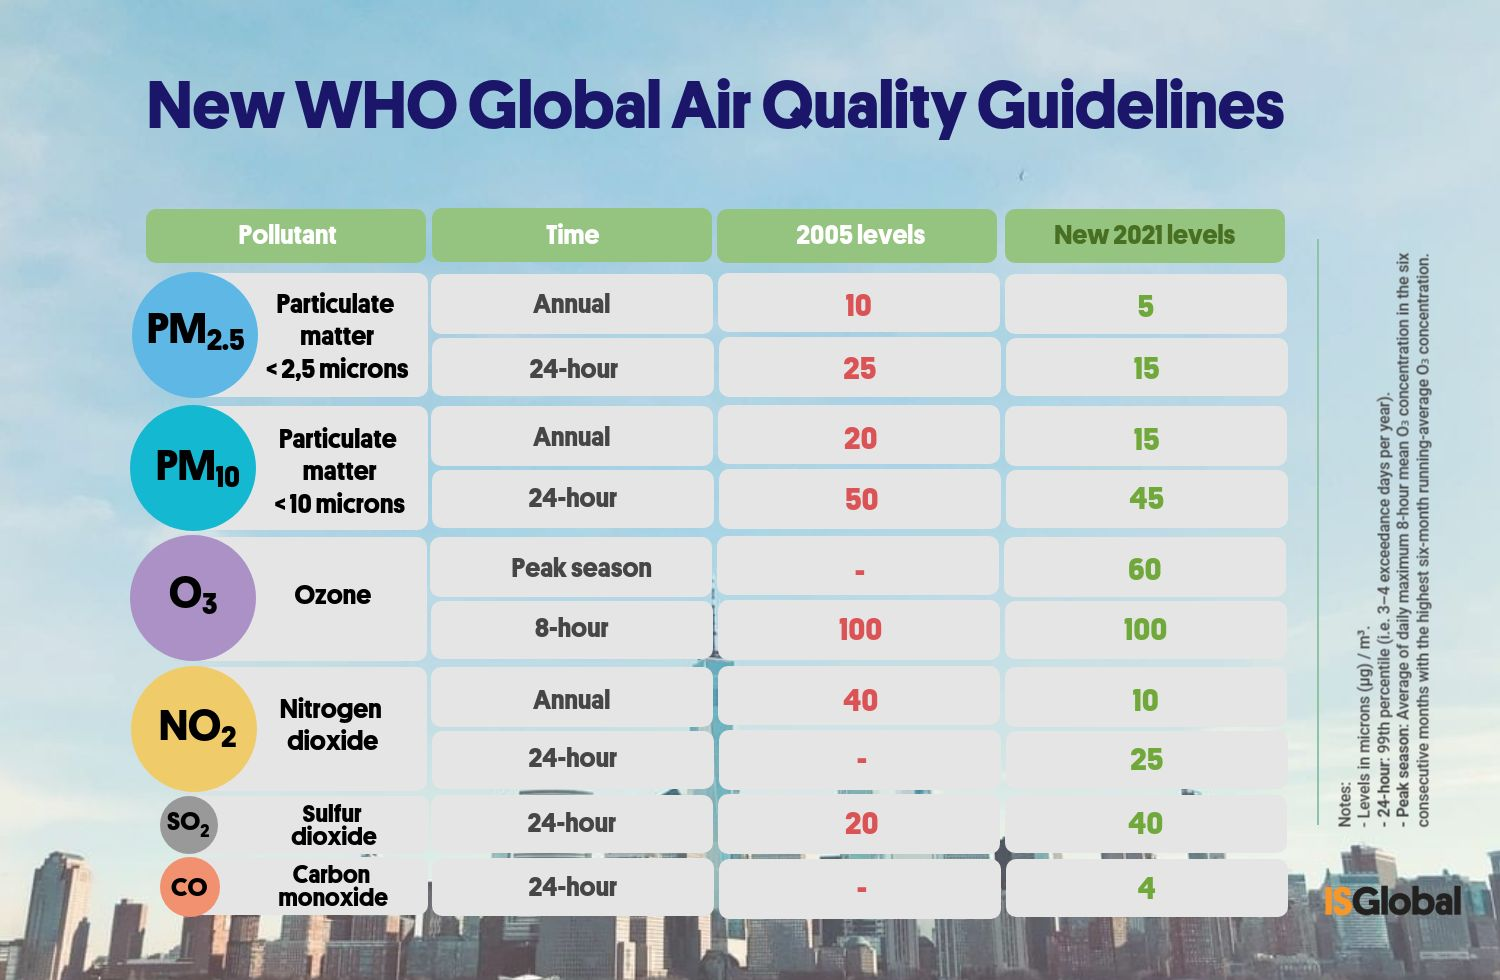
\includegraphics[width=0.8\textwidth]{εικόνες/directrices calidad aire OMS eng.jpg}
    \caption{Οι παγκόσμιες οδηγίες του Π.Ο.Υ για την ποιότητα του αέρα \cite{Nieuwenhuijsen2021}}
    \label{fig:WhoGuidelines}
\end{figure}

\FloatBarrier


